\documentclass{article}
\usepackage{pgfplots}
\pgfplotsset{compat=1.16}

\begin{document}

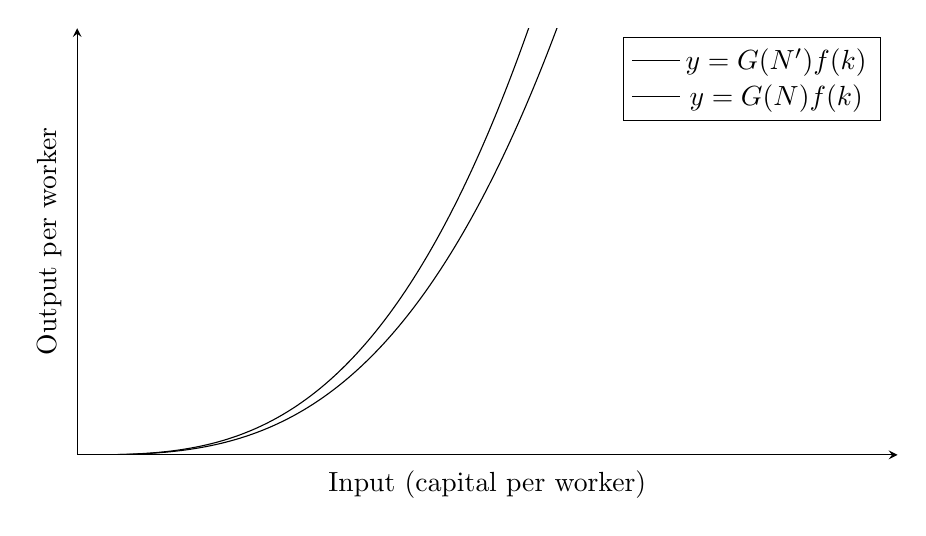
\begin{tikzpicture}
    \begin{axis}[
        axis lines=left,
        xlabel={Input (capital per worker)},
        ylabel={Output per worker},
        ymin=0, ymax=5,
        xmin=0, xmax=5,
        ytick=\empty,
        xtick=\empty,
        enlargelimits=false,
        height=7cm,
        width=12cm,
        title style={at={(0.5,1.0)}, anchor=south,yshift=-0.5ex},
        ]
        \addplot[smooth, domain=0:4.5,samples=100] {0.2*(x^3)};
        \addlegendentry{$y = G(N')f(k)$}
        \addplot[smooth, domain=0:4.5,samples=100] {0.2*(1.2*x^3)};
        \addlegendentry{$y = G(N)f(k)$}
    \end{axis}
\end{tikzpicture}

\textbf{External economies of agglomeration as experienced by a firm through a shift in the production function due to an increase in the size of a city ($N$ to $N'$).}

\end{document}